\chapter{Appendix-A Calculation of the bearing resistance}
\label{app1}
\onehalfspacing


% Example text
%https://en.wikipedia.org/wiki/Bearing_pressure wait zhuan xie

\section{Equivalent bearing stress area}

We know that when a cylinder and another almost equal diameter cylindrical hole into the bearing state, for the contacted plate, the range of bearing stress should be Fig. \ref{fig-shce-bea} in the shaded part of the drawing line, which is pressurized by the actual range of contact for the arc length $s$ multiplied by the thickness of the plate $t$, however, the actual calculating in the engineering, generally do not take into account the length of the arc, and the calculation of the cylindrical axis of the bearing stress to calculate the equivalent area of bearing and the equivalent effect of the force.

\begin{figure}[htbp]
    \centering
    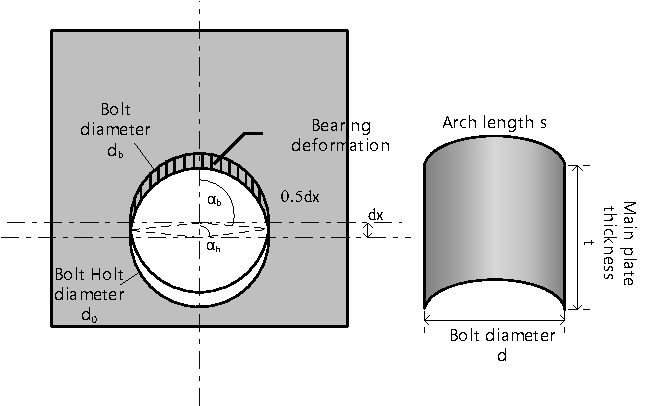
\includegraphics[width=0.8\textwidth]{imgs/app/shce-bea.pdf}
    \caption{Schematic diagram of bearing stress}
    \label{fig-shce-bea}
\end{figure}

The equivalent bearing stress can be calculated by the following equation:

\begin{equation}
    f_{be} = \frac{P}{d \times t}
\end{equation}


As in Fig. \ref{fig-eqvbea}, it is assumed here that the shaft portion inside the cylinder is subjected to uniform hydrostatic pressure, and the combined force of the equivalent area of hydrostatic pressure (i.e., the cross-section of the shaft portion) should at this point be equal to the combined force of the bearing stresses on the half circumference of the borehole wall (i.e., the general arc length $s$), which can be expressed as the following equation:

\begin{equation}
    dtf_{be} = \sum_0^s t f_b
\end{equation}

\begin{figure}[htbp]
    \centering
    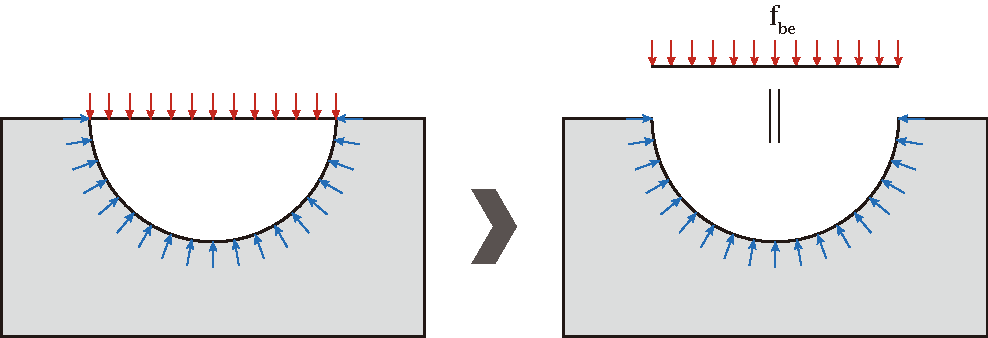
\includegraphics[width=0.8\linewidth]{imgs//app/eqvbea.pdf}
    \caption{Schematic of equivalent bearing stress area}
    \label{fig-eqvbea}
\end{figure}


As in Fig. \ref{fig-calcuequ}, the arc length is $s$ and the angle of rotation $\theta$. Within an arc length region $ds$ of a tiny angle of rotation $d\theta$, the combined force in this tiny region can be computed as the following equation:

\begin{equation*}
    dP_{xy}=f_b \times ds \times t = 0.5 \times d \times t \times f_b \times d\theta
\end{equation*}

At this point the tiny combined force is pointing towards the center o of the circle, which needs to be converted to the direction of the force, that is, the y-direction, and the y-direction component force can be calculated as follows:

\begin{equation*}
    dP_y= cos(\theta) dP_{xy} = 0.5 \times cos(\theta) f_b \times d \times t \times d\theta
\end{equation*}

For the x-direction component force $dP_x$, which is ultimately symmetric to the y-axis, it will cancel out and annihilate with the x-negative direction component force $dP_{-x}$, so it doesn't need to be considered further.

Ultimately, integrating all the tiny y-direction combined forces, the y-direction bearing force $P$ can be calculated as:

\begin{align*}
    P_y &= \int_{-\pi / 2}^{-\pi / 2} 0.5 \times d \times t \times f_b \times cos(\theta) \times d\theta \\
    &=0.5 \times f_b \times d \times t \times[\sin (\theta)]_{-\pi / 2}^{\pi / 2} \\
    &= d \times t \times f_b
\end{align*}

    

\begin{figure}[htbp]
    \centering
    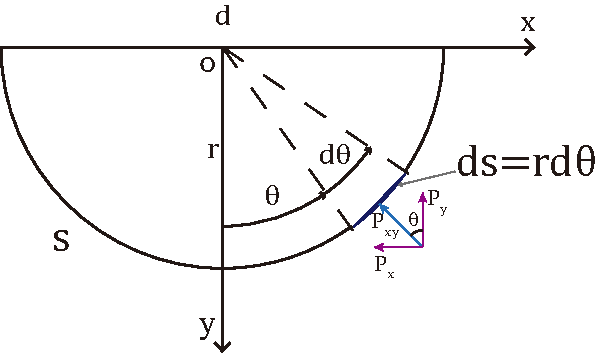
\includegraphics[width=0.5\linewidth]{imgs//app/calcubea.pdf}
    \caption{Calculation of equivalent bearing stress}
    \label{fig-calcuequ}
\end{figure}


Therefore for the calculation method of bearing resistance of the connection, it can be calculated according to the equivalent stress region. However there will still be areas of stress concentration, which will be discussed in the next section.

\section{Investigate the effective bearing area for pin}


The design of the pin joint is considered to be a contact problem between the cylinder and the cylindrical groove, as shown in Fig. \ref{fig:cycon}. The mechanism of load transfer by this bearing pressure is the same as that of a high-strength bolt. On the other hand, in the road standards, Hertz's contact was considered for the bearing design of pins. The design equations for each standard are summarized as follows:

\begin{figure}[htbp]
    \centering
    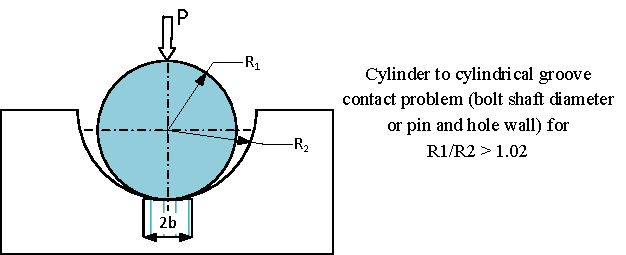
\includegraphics[width=0.9\textwidth]{imgs/app/cylinders-contact.pdf}
    \caption{Contact between cylinder and cylindrical groove}
    \label{fig:cycon}
\end{figure}

In AASHTO \cite{AASHTO2020}, the bearing capacity of Pin is shown in the following equation. Note that with AASHTO, the coefficient of Pin wear can be reduced from 1.5 to 0.75, half of the original coefficient.

    \begin{equation}
        (R_{pB})_r = \Phi_b(R_{pB})_n = \Phi_b \times 1.5td_1F_y
    \end{equation}
Where, $t$ is the thickness of main plate,$d_1$: the diameter of Pin, $\Phi_b$: bearing resistance coefficient($\Phi_b = 1$) 

Eurocode 3 \cite{eurocode3-21}, it is assumed that the pin bearing stresses are evenly distributed on the shaft of the pin. The bearing stresses must satisfy the following equations.

    \begin{equation}
        \sigma_{h,Ed} 	\leq f_{h,Rd}
    \end{equation}
Where,
    \begin{equation}
        \sigma_{h, \mathrm{Ed}}=0.591 \sqrt{\dfrac{E F_{b, E d, s e r}\left(d_{0}-d_1\right)}{d_1^{2} t}}
    \end{equation}
    \begin{equation}
        f_{h,Rd} = 2.5f_y/\gamma_{M6,ser}
    \end{equation}

Where, $d_1$: is the diameter of the pin, $d_0$: is the diameter of the hole, $F_{b,Ed,ser}$: design bearing resistance for serviceability limit state.

The design bearing capacity on the Eurocode 3 resisting side is shown in the following equation.

    \begin{equation}
        \text{For SLS: } F_{b,Rd,ser} = 0.6td_1 f_y/\gamma_{M6,ser} \geq F_{b,Ed,ser}
    \end{equation}
    \begin{equation}
        \text{For ULS: } F_{b,Rd} = 1.5td_1 f_y/\gamma_{M0} \geq F_{b,Ed}
    \end{equation}
Where, $F_{b,Rd}$: bearing resistance, $F_{b,Ed}$: Working side bearing strength considering Hertz equation, $\gamma_{M0}$: Partial safety rate.

The bearing capacity can be calculated by specifying the allowable bearing stress. From the explanation of allowable bearing capacity, the description is divided into surface contact (when a flat surface contacts a flat surface) and Hertz contact \cite{hertz1882Ueber} (when a curved surface contacts a curved surface or a curved surface contacts a flat surface within a very small range). When $pin hole r_1 / pin radius r_2$ is less than 1.02, the entire cross section of the pin is considered to be in contact with the bore wall, and the contact pressure is equally distributed over the projected area of the pin. When $r_1 / r_2$ exceeds 1.02, Hertz's formula\ref{eq.hertz1} is used.

\begin{equation}
\begin{cases}
\text{Diameter for curvature: } &\frac{1}{d^*} = \frac{1}{d_1} +\frac{1}{d_2} \\

\text{Elasticity of elasticity: } &\frac{1}{E^*} = \frac{(1-\nu_1^2)}{E_1}+\frac{(1-\nu_2^2)}{E_2} \\

\text{Contact surface width: } & b=  (\frac{2F}{\pi L} \cdot \frac{d^*}{E^*})^{1/2}

\end{cases}  
\label{eq.hertz1}
\end{equation}

Where $d_1$: shaft diameter, $d_2$: pore diameter, $d_*$: curvature relative diameter, $\nu_1$: Poisson's ratio of fastener, $\nu_2$: Poisson's ratio of bonded material,$E_1$: elastic modulus of fastener, $E_2$: elastic modulus of bonded material, $E^*$: equivalent elastic modulus, $F$: bearing force, $L$: shaft length. \par

The maximum contact pressure considering the Hertz formula is shown in following equation.

\begin{equation}
   P_{max} = \dfrac{2F}{\pi b L} = \sqrt{\dfrac{2FE^*}{\pi Ld^*}}
\end{equation}


The maximum stress appears at the center of the contact position between the cylinder and the groove from the Hertz contact. This maximum stress is shown in the following equation\ref{eq-sigmamax} \cite{g1979AideMemoire}.

\begin{equation}
    \sigma_{3}=-\left|\sigma_{\max }\right|=0.5642 \times \sqrt{\dfrac{P}{l} \cdot \dfrac{\dfrac{R_{2}-R_{1}}{R_{1} \cdot R_{2}}}{\dfrac{1-\mu_{1}^{2}}{E_{1}}+\dfrac{1-\mu_{2}^{2}}{E_{2}}}}
    \label{eq-sigmamax}
\end{equation}

If $E_1 = E_2 = E ; \nu_1 = \nu_2 = 0.3$, so called, and the fastener and the material to be joined are of the same material, the above equation can be transformed as follows:

\begin{equation}
    \sigma_{\max }=0.418 \times \sqrt{\dfrac{P}{l} \cdot \dfrac{R_{2}-R_{1}}{R_{1} \cdot R_{2}} \cdot E}
    \label{eq-sigmamax2}
\end{equation}

The width b at this time can be calculated from the following equation \ref{eq-hertzb2}: \par

\begin{equation}
    b=1.128 \times \sqrt{\dfrac{P}{l} \cdot \frac{R_{1} \cdot R_{2}}{R_{2}-R_{1}}\left(\dfrac{1-\mu_{1}^{2}}{E_{1}}+\dfrac{1-\mu_{2}^{2}}{E_{2}}\right)}
    \label{eq-hertzb2}
\end{equation}

Since the fastener and the material to be joined are the same steel and have close modulus of elasticity, the equation can be transformed as follows:

\begin{equation}
    b=1.522 \times \sqrt{\dfrac{P}{l \cdot E} \cdot \dfrac{R_{1} \cdot R_{2}}{R_{2}-R_{1}}}
    \label{eq-hertzb3}
\end{equation}



\section{Investigate the Shaft Diameter/Hole Diameter}

Comparison of design bearing stresses for each design standard are shown in Fig. \ref{fig-baecoefficient}.
For the bolt bearing connection at this stage, only the Japanese \ac{JSHB} adopts the use of limit design, however, its calculation formula is used through the previous \ac{ASD} design method, the author believes that this formula is too high evaluation of the use of limit strength of the bearing resistance of the bearing connection, in the long term cyclic loading will be deformed holes, resulting in the emergence of a larger gap, so that it loses its original bearing state, it should be referred to for the The author believes that this formula overestimates the service limit strength of the bearing connection, and the hole will deform under long-term cyclic loading, resulting in a larger gap, making it lose its original pressure-bearing state, and should be referred to the design for the service limit of the pin for a safer evaluation of the bearing connection, because the bearing hole is not allowed to plastic deformation under long-term round-trip loading.

\begin{figure}[htbp]
    \centering
    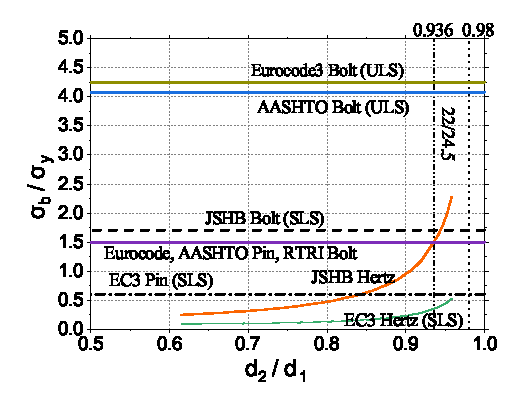
\includegraphics[width=0.7\textwidth]{imgs/app/eachcode-fb.eps}
    \caption{Comparison of design bearing stresses for each design standard}
    \label{fig-baecoefficient}
\end{figure}    

% The bearing capacity design equations for each standard are shown in Figure ϭref{fig-baecoefficient}. Since the above equations are based on both the allowable stress design method and the limit state design method, $F_u$ in the Eurocode or AASHTO ultimate state is converted to $\sigma_y$ for ease of comparison. Here, the material to be welded is assumed to be ss400, and the yield point and tensile strength are assumed to be 235 $N/mm^2$ and 400 $N/mm^2$, respectively. \cH00000000000000}
%  In Erucode, the pin design was divided into the limit state of use and the end state. The design condition is satisfied if the design bearing capacity on the resisting side (dotted line Eur Pin Ser) is greater than the bearing strength on the acting side (Eur Hertz Ser). The M22 bolt most commonly used in bridges has a standard hole diameter of 24.5, and its $d_2/d_1$ is 0.936 (two dashed lines in the figure), the Eur Pin Ser on the resisting side is greater than the Eur Hertz Ser on the acting side, so the design was made on the safe side. On the other hand, since the applicable range of the Hertz equation is $d_2/d_1 < 0.98$, the closer to the applicable range of the Eurocode bearing capacity design equation, the closer to the design bearing capacity on the resisting side and the strength on the acting side. \par
% In AASHTO, the pin or bolt bearing design was designed without considering the Hertz equation, and the bearing design capacity of the bolt and pin was designed with 2.4 and 1.5$sigma_yd_1t$, respectively. \sigma_yd_1t$}
% In the specification for road bridge, the design bearing capacity of pin joints was designed by considering the Hertz equation. The bolts were designed with $1.7\sigma_y$, and if the value is larger than $d_2/d_1=0.944$, the bearing capacity is smaller than the bearing capacity formula for pins, and the evaluation was made on the safe side. \par
% The design bearing capacity limit stress of the joints in AASHTO and Eurocode can be larger than that in Europe and the U.S. because the design bearing capacity limit stress of the joints in AASHTO and Eurocode can be larger than that in Europe and the U.S. according to the joint shape and bolt arrangement. However, the design of service limit state of bearing joints with support bolts has not been considered. \par

\section{Effect of the plate thicknesses}

%ファスナーの支圧接触は基本接触断面が全断面有効に接触すると仮定して幅方向に一様な分布を有した直応力を求められた.しかしながら,これはあくまでも初等はり理論の仮定として,実際にファスナーの境界条件や形状によって影響する.その影響を無視できない範囲に至れば結局一様な直応力分布を仮定しにくい.図\ref{fig-bshearlag}に示すように,被接合材の板厚が極厚の場合には,被接合材の中央接触範囲で直応力を有効に伝達出来ず,両側に分布している.この応力分布は箱断面フランジでよく発生するせん断遅れ(shear lag)とよく類似している.\par
%板厚に関する基準では,道示やAASHTOが特に決めていないが,図\ref{fig-bshearlag}の右の示すようにEurocodeでは締付長さlが$3d_1$を超えた場合は接触の直応力が両側$1.5d_1$の有効範囲を決めた.\par

The direct stresses with uniform distribution in the width direction were obtained by assuming that the basic contact section of the fastener is in effective contact with the entire cross section. However, this is only an assumption of elementary beam theory, and is affected by the actual boundary conditions and geometry of the fastener. If the influence is not negligible, it is difficult to assume a uniform distribution of direct stresses. As shown in Fig. \ref{fig-bshearlag}, when the thickness of the material to be joined is extremely thick, the direct stresses cannot be effectively transferred in the central contact area of the material to be joined, and are distributed on both sides. This stress distribution is similar to the shear lag that often occurs in box flanges.

In terms of the standard for plate thickness, the road standard and AASHTO have not specifically determined the effective range of direct contact stresses of $1.5d_1$ on both sides when the clamping length l exceeds $3d_1$, as shown on the right side of Fig. \ref{fig-bshearlag} in the Eurocode 3.

\begin{figure}[htbp]
 \centering
 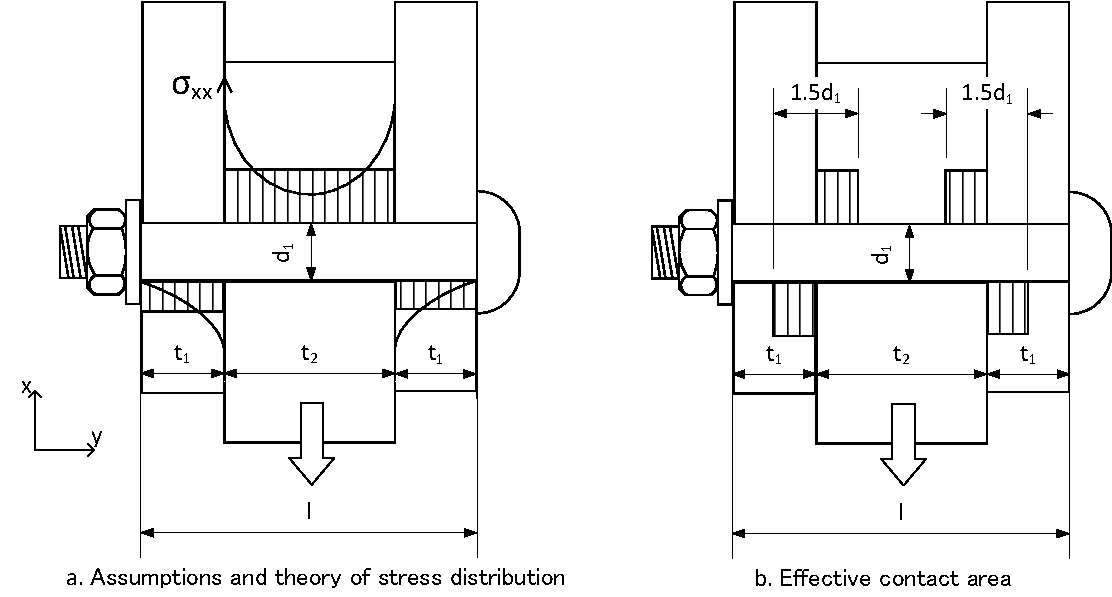
\includegraphics[width=0.8\textwidth]{imgs/app/boltlength-sl.pdf}
 \caption{Straight stress distribution caused by long tightening length}
 \label{fig-bshearlag}
\end{figure}

